\begin{minipage}[t]{170mm}
\vspace{3mm}
\section*{Guide til at finde sig selv}
Når du på et tidspunkt er forsvundet, og ikke ved hvor du er, så er her en guide:

Se på den nærmeste dør. Noter det navn døren har, fx G32, D.01 eller KollG3. Bogstaverne henviser til hvilken gang du befinder dig på. Se kortet nedenfor. Nu finder du en trappe og bevæger dig ned i stueplan. Nu burde du være på kendt territorie og kan følge din egen stedsans eller de $69$ pile, tilbage til der hvor du burde være.
\begin{center}
%$\quad$\hspace{4cm}
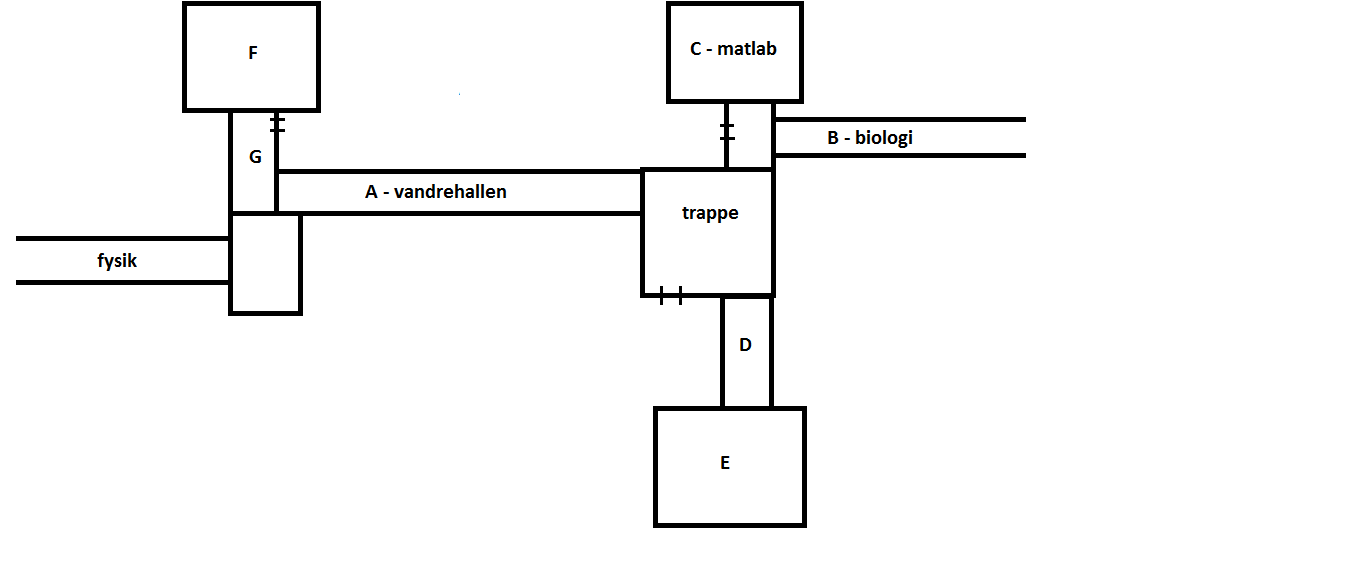
\includegraphics[width=1.2\linewidth]{bogstav-kort.png}
\end{center}
\vspace{-9mm}
\section*{Ikke-kommutativ studenterrådgivning}
\emph{Kære brevkasse}

\emph{Min ven fortæller mig, at medmindre man har set på noget i mere end $4$ sekunder, så må man ikke udtale sig om hvordan det ser ud.}

\emph{Jeg forstår det ikke. Hvorfor?}

\emph{Hilsen den forundrede, der ser noget i 2,25 sekunder}

\subsection*{Svar}
Kære forundrede

Jeg må desværre advare dig, da dit brev peger på at du færdes i uheldige kredse, og din ven måske ikke er så godt selskab, som du tror. At du læser dette ansete dagblad, peger jo tydelig på at du har en naturvidenskabelig baggrund og det er derfor nok med at se noget i omtrent $5.39 \cdot 10^{-44}$ sekunder før du har retten til at udtale dig om det. Forvirringen optræder, fordi din "ven"\ er humanist og som følge af en resolution, vedtaget af videnskabernes selskab i 1777 må humanister ikke udtale sig om ting, de har set i mindre end fire sekunder. Den oprindelige begrundelse for dette forbud, var at man ville få humanisterne til at holde kæft, men sidenhen har reglen udviklet sig til en grundpile i nordens videnskabelige diskurs, da tværfaglige forhandlinger i uddannelsessystemet sidenhen ofte tager $3.9$ og afsluttes med, at rette videnskabsfolk bliver enig om, at enhver løsning er bedre end at lade humanisten komme til orde, noget der har øget effektiviteten mere, end sprogets indførelse for $2$ millioner år siden. 

Så konklusionen må være, at du kan udtale om enhver ting, du er i stand til at observere, men at du bør finde dig nogle rigtige venner, som ikke presser dig mod undergangen.

{\flushright\emph{Hilsen den ikke-kommutative studenterrådgivning}}

\vspace{1mm}

\section*{Dagens digt -- Hellig er maskinen}
\begin{center}
Keats løfter sit åsyn og ser superstærkt på turtelduen, thi når kirkeklokkerne ringer, vil turtelduen segne i dyb afmagt foran den veltalende løjtnant, og Keats harmes derved.

Sky de elskende. For de vil drikke gammel mælk med Gauss' svaner ved Eulers krybbe når dagen dør.

Den, der i sandhed elsker Galois, bør drage langt bort med de ævlende politibetjente hver søndag.

Skal jeg end vandre i Legoland, vil klovnene ej gå til gudstjeneste med mig; thi Galois er med mig.
\end{center}

\end{minipage}
